% 浙江大学博士学位论文 — 阿秒电子显微术
% Template: zjuthesis v10.0.1
% Test generated by bishe-guider pipeline

\documentclass[
    PrintFilePath   = false,
    TwoSide         = true,
    StudentName     = 姓名,
    StudentID       = 学号,
    AdvisorName     = 指导教师,
    Grade           = 2020,
    Major           = 光学工程,
    Department      = 光电科学与工程学院,
    SubmitDate      = 2026-06-01,
    MajorFormat     = opteng,
    Degree          = graduate,
    Type            = thesis,
    Period          = final,
    BlindReview     = false,
    Language        = chinese,
    GradLevel       = doctor,
    Topic           = 超快光学,
    ColaboratorName = 合作导师,
    ListOfContents  = true,
    ListOfFigures   = true,
    ListOfTables    = true,
    ListOfAlgorithms= false,
    Title           = 阿秒电子显微术——亚周期光场动力学的高时空分辨成像,
    TitleEng        = {{Attosecond Electron Microscopy --- High Spatiotemporal Resolution Imaging of Sub-Cycle Optical Field Dynamics}}
]{zjuthesis}

\usepackage{amsmath,amssymb}
\usepackage{graphicx}
\usepackage{booktabs}
\usepackage{siunitx}
\usepackage{physics}

\graphicspath{{figures/}{figure/}}
\addbibresource{references.bib}

\begin{document}

\coverstyle
\inputpage{cover}

\prevstyle
\inputpage{previous}
\inputpage{toc}

\bodystyle

% ===== 第1章 绪论 =====
% 第1章 绪论
\chapter{绪论}
\label{chap:intro}

\section{研究背景与意义}
\label{sec:bg}

光与物质的相互作用是现代物理学的核心议题之一。在纳米尺度上，电磁场在单个光学周期内经历复杂的时间演化过程，其特征时间尺度为飞秒（$\SI{1}{fs} = 10^{-15}\;\text{s}$）量级，特征空间尺度为纳米至亚纳米量级。理解并直接测量这一时空尺度上的电磁场分布$\mathbf{E}(\mathbf{r}, t)$，对于纳米光子学、超快光谱学和量子光学等领域具有重要的科学意义。

传统的光学测量方法受到衍射极限的制约，空间分辨率被限制在半波长量级（$\sim\lambda/2$）。以可见光波段为例，800\,nm波长的光其衍射极限约为400\,nm，远远无法满足纳米尺度空间分辨的需求。近场光学技术（如散射型扫描近场光学显微镜，s-SNOM）可将空间分辨率提升至$\sim\SI{10}{nm}$，但其时间分辨率受限于探测脉冲的持续时间，通常为数十飞秒，不足以分辨单个光场周期内的动力学过程。

电子显微镜在空间分辨率方面具有天然优势。keV能量的电子具有皮米（$\SI{1}{pm} = 10^{-12}\;\text{m}$）量级的德布罗意波长，远超光学衍射极限。然而，传统超快电子显微术的时间分辨率受限于电子脉冲宽度，由于库仑排斥和空间电荷效应，脉冲宽度停留在$\sim\SI{100}{fs}$，比可见光的光学周期（$\sim\SI{2.7}{fs}$ @ 800\,nm）长两个数量级。这一"时间分辨率的鸿沟"阻碍了对亚周期电磁动力学的直接观测。

阿秒科学的兴起为突破这一时间壁垒提供了全新的工具。2001年，Hentschel等人\cite{Hentschel2001}和Drescher等人\cite{Drescher2001}首次在实验上产生了孤立阿秒脉冲，打开了亚飞秒时间分辨的大门。2023年诺贝尔物理学奖授予Agostini、Krausz和L'Huillier三位科学家，以表彰他们在阿秒脉冲产生方面的开创性贡献\cite{nobel2023}。然而，光子基的阿秒探针受制于光波长的衍射极限，即使在30\,nm的软X射线波段，空间分辨率也仅能达到$\sim\SI{15}{nm}$——比keV电子的皮米级分辨率粗糙三个数量级。

本文所研究的阿秒电子显微术，将阿秒科学的时间分辨能力与电子显微镜的空间分辨能力有机结合，填补了超快科学中高时空分辨测量的关键空白。图\ref{fig:ch1-resolution-map}展示了不同超快测量技术在时间-空间分辨率图上的定位。

\begin{figure}[htbp]
    \centering
    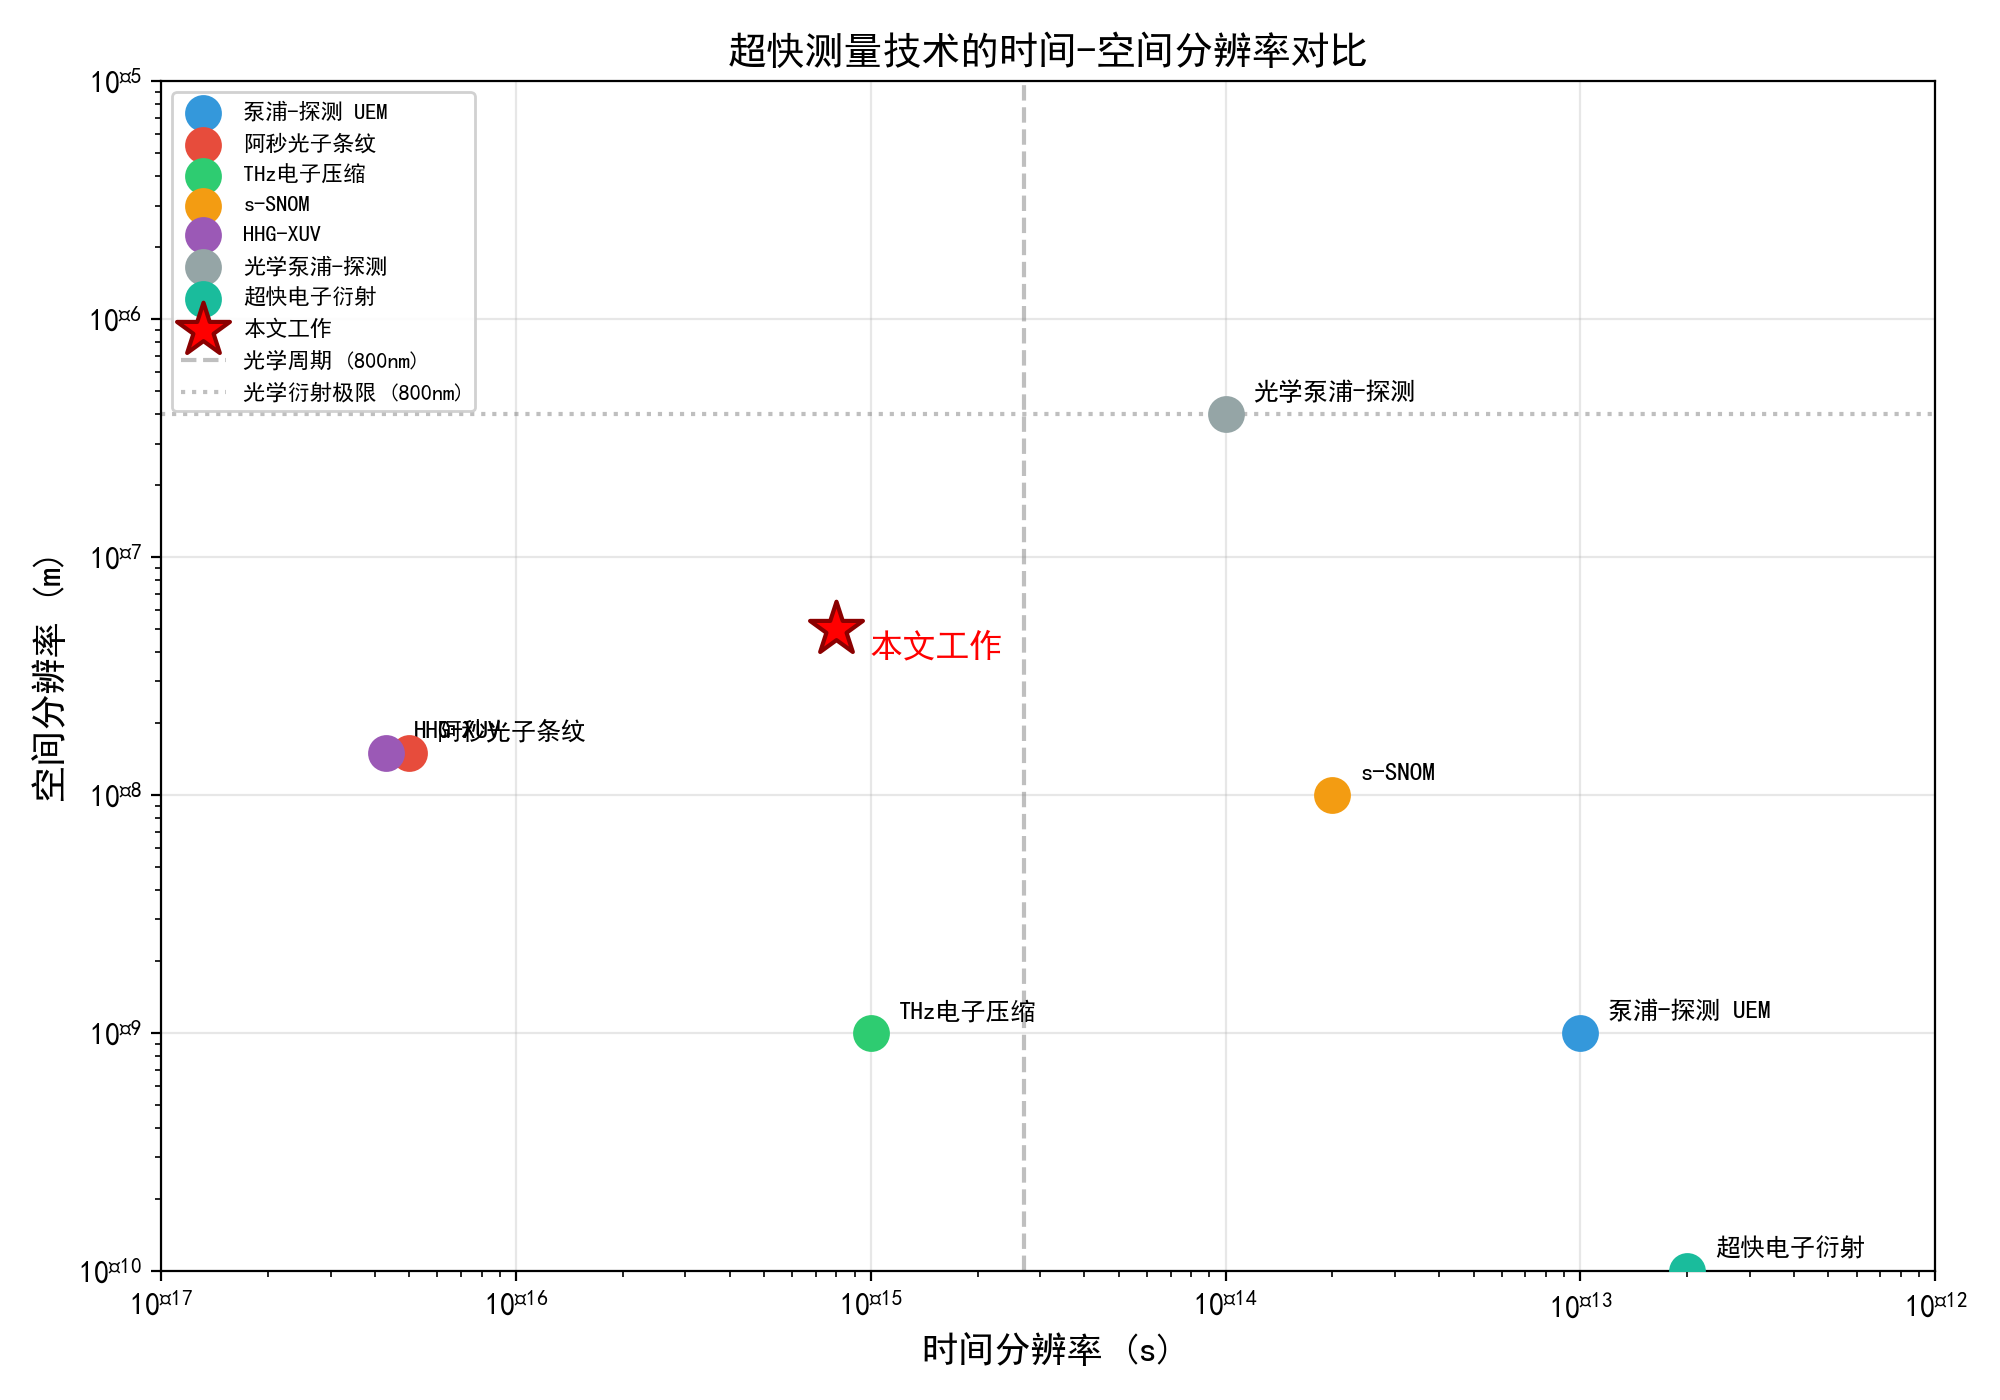
\includegraphics[width=0.85\linewidth]{ch1/fig_resolution_map}
    \caption{\label{fig:ch1-resolution-map} 超快测量技术的时间-空间分辨率对比。横轴为时间分辨率，纵轴为空间分辨率。阿秒电子显微术（红色星号）位于时间分辨率$\sim\SI{800}{as}$、空间分辨率$\sim\SI{50}{nm}$的独特位置，填补了光子探针和电子探针之间的空白。}
\end{figure}

\section{超快电子显微术的发展}
\label{sec:uem-dev}

超快电子显微术的发展可追溯至Zewail课题组在2000年代初的开创性工作。Zewail等人\cite{Zewail2010}建立了四维电子显微术（4D electron microscopy），利用飞秒激光触发泵浦-探测方案，在透射电子显微镜中实现了$\sim\SI{1}{nm}$空间分辨率和$\sim\SI{100}{fs}$时间分辨率的联用。这一技术使得对结构动力学（如相变、晶格振动、化学反应中间态）的实时观测成为可能。

然而，泵浦-探测型超快电子显微术面临两个根本性限制。第一，电子脉冲的时间展宽：由于电子之间的库仑排斥效应（空间电荷效应），飞秒电子脉冲在传播过程中不可避免地展宽，即使在单电子模式下，脉冲宽度也受到初始能量弥散的限制。第二，时间分辨率的不对称性：时间分辨率受限于泵浦脉冲和探测脉冲中较长的一个，且无法突破光学周期的限制。

针对上述限制，研究者发展了多种电子脉冲压缩技术。Baum和Zewail\cite{Baum2007}提出了利用射频腔对电子脉冲进行时间压缩的方案。Ryabov和Baum\cite{Ryabov2016}利用太赫兹脉冲驱动的电子脉冲压缩，实现了$\sim\SI{1}{fs}$的时间分辨率，并实现了电磁波波形的直接成像。

近年来，超快透射电子显微镜（UTEM）技术也取得了重要进展。Feist等人\cite{Feist2015}在UTEM中实现了光控电子量子态的相干调制，证明了自由电子与光场之间的量子相干相互作用。这一工作为光场驱动的电子波函数操控奠定了实验基础。

\section{阿秒科学的产生与进展}
\label{sec:attosecond-dev}

阿秒科学的根基在于高次谐波产生（high-harmonic generation, HHG）现象。1993年，Corkum\cite{Corkum1993}提出了著名的三步模型（three-step model），将强场电离过程分解为隧道电离、自由电子在激光场中的加速运动、以及电子与母离子的复合辐射三个阶段。这一模型定量解释了HHG的平台区和截止频率，为阿秒脉冲的产生提供了理论指导。

Antoine等人\cite{Antoine1996}从理论上预言了利用HHG产生阿秒脉冲串的可能性。2001年，两个研究组分别在实验上实现了阿秒脉冲的产生和表征：Hentschel等人\cite{Hentschel2001}产生了$\sim\SI{650}{as}$的脉冲，Drescher等人\cite{Drescher2001}实现了$\sim\SI{2.7}{fs}$的软X射线脉冲。这些突破性进展标志着阿秒科学的正式诞生。

Krausz和Ivanov\cite{Krausz2009}在2009年的综述中系统总结了阿秒物理的发展，指出了阿秒脉冲在原子分子动力学观测中的广泛应用前景。随后，阿秒脉冲的持续时间被不断缩短，目前已达到$\sim\SI{43}{as}$的最短记录\cite{Li2020_as}。在空间分辨率方面，Popmintchev等人\cite{Popmintchev2012}将HHG扩展到keV硬X射线波段，为高能量阿秒光子提供了可能。

阿秒科学的应用范围也在不断扩大。从最初的原子物理（电子隧穿观测\cite{Uiberacker2007}），到分子动力学（电子定位\cite{Sansone2010}），再到凝聚态物理（超快退磁\cite{Kirilyuk2010}），阿秒技术正在向越来越多的学科渗透。Varillas等人\cite{Varillas2026}在2026年的阿秒科学路线图中展望了未来十年的发展方向，强调了阿秒技术与电子显微术结合的重要潜力。

\section{阿秒电子显微术的提出与科学问题}
\label{sec:proposal}

阿秒电子显微术的核心理念是将阿秒级时间结构"刻印"到电子束中，使电子束自身成为阿秒时间分辨的探针。这一思想的理论基础源于Tsarev、Ryabov和Baum\cite{Tsarev2021}提出的时间Talbot效应：连续波激光对电子波函数进行周期性能量调制后，电子在自由空间传播过程中会经历Talbot回复，在特定传播距离处形成阿秒级时间宽度的电子脉冲串。

与传统泵浦-探测方案不同，这一方法不需要飞秒激光器：一束连续波（continuous-wave, CW）激光即可产生阿秒电子脉冲。这一特点大大降低了实验复杂度，同时从根本上避免了空间电荷效应导致的脉冲展宽——因为每个光学周期内最多只有一个电子通过样品。

本文聚焦于以下科学问题：

\begin{enumerate}
    \item 如何利用连续波激光在常规透射电子显微镜中产生可调控的阿秒电子脉冲？
    \item 阿秒电子脉冲如何实现对纳米结构近场的亚周期时间分辨成像？
    \item 手性纳米结构中的表面波动力学在亚周期尺度上呈现怎样的特征？
    \item 介质纳米共振器中不同阶 Mie 模式之间的时间延迟是否可以直接观测？
    \item 纳米加工精度如何影响多天线系统的电磁响应对称性？
\end{enumerate}

图\ref{fig:ch1-framework}展示了本文的研究框架和各章节之间的逻辑关系。

\begin{figure}[htbp]
    \centering
    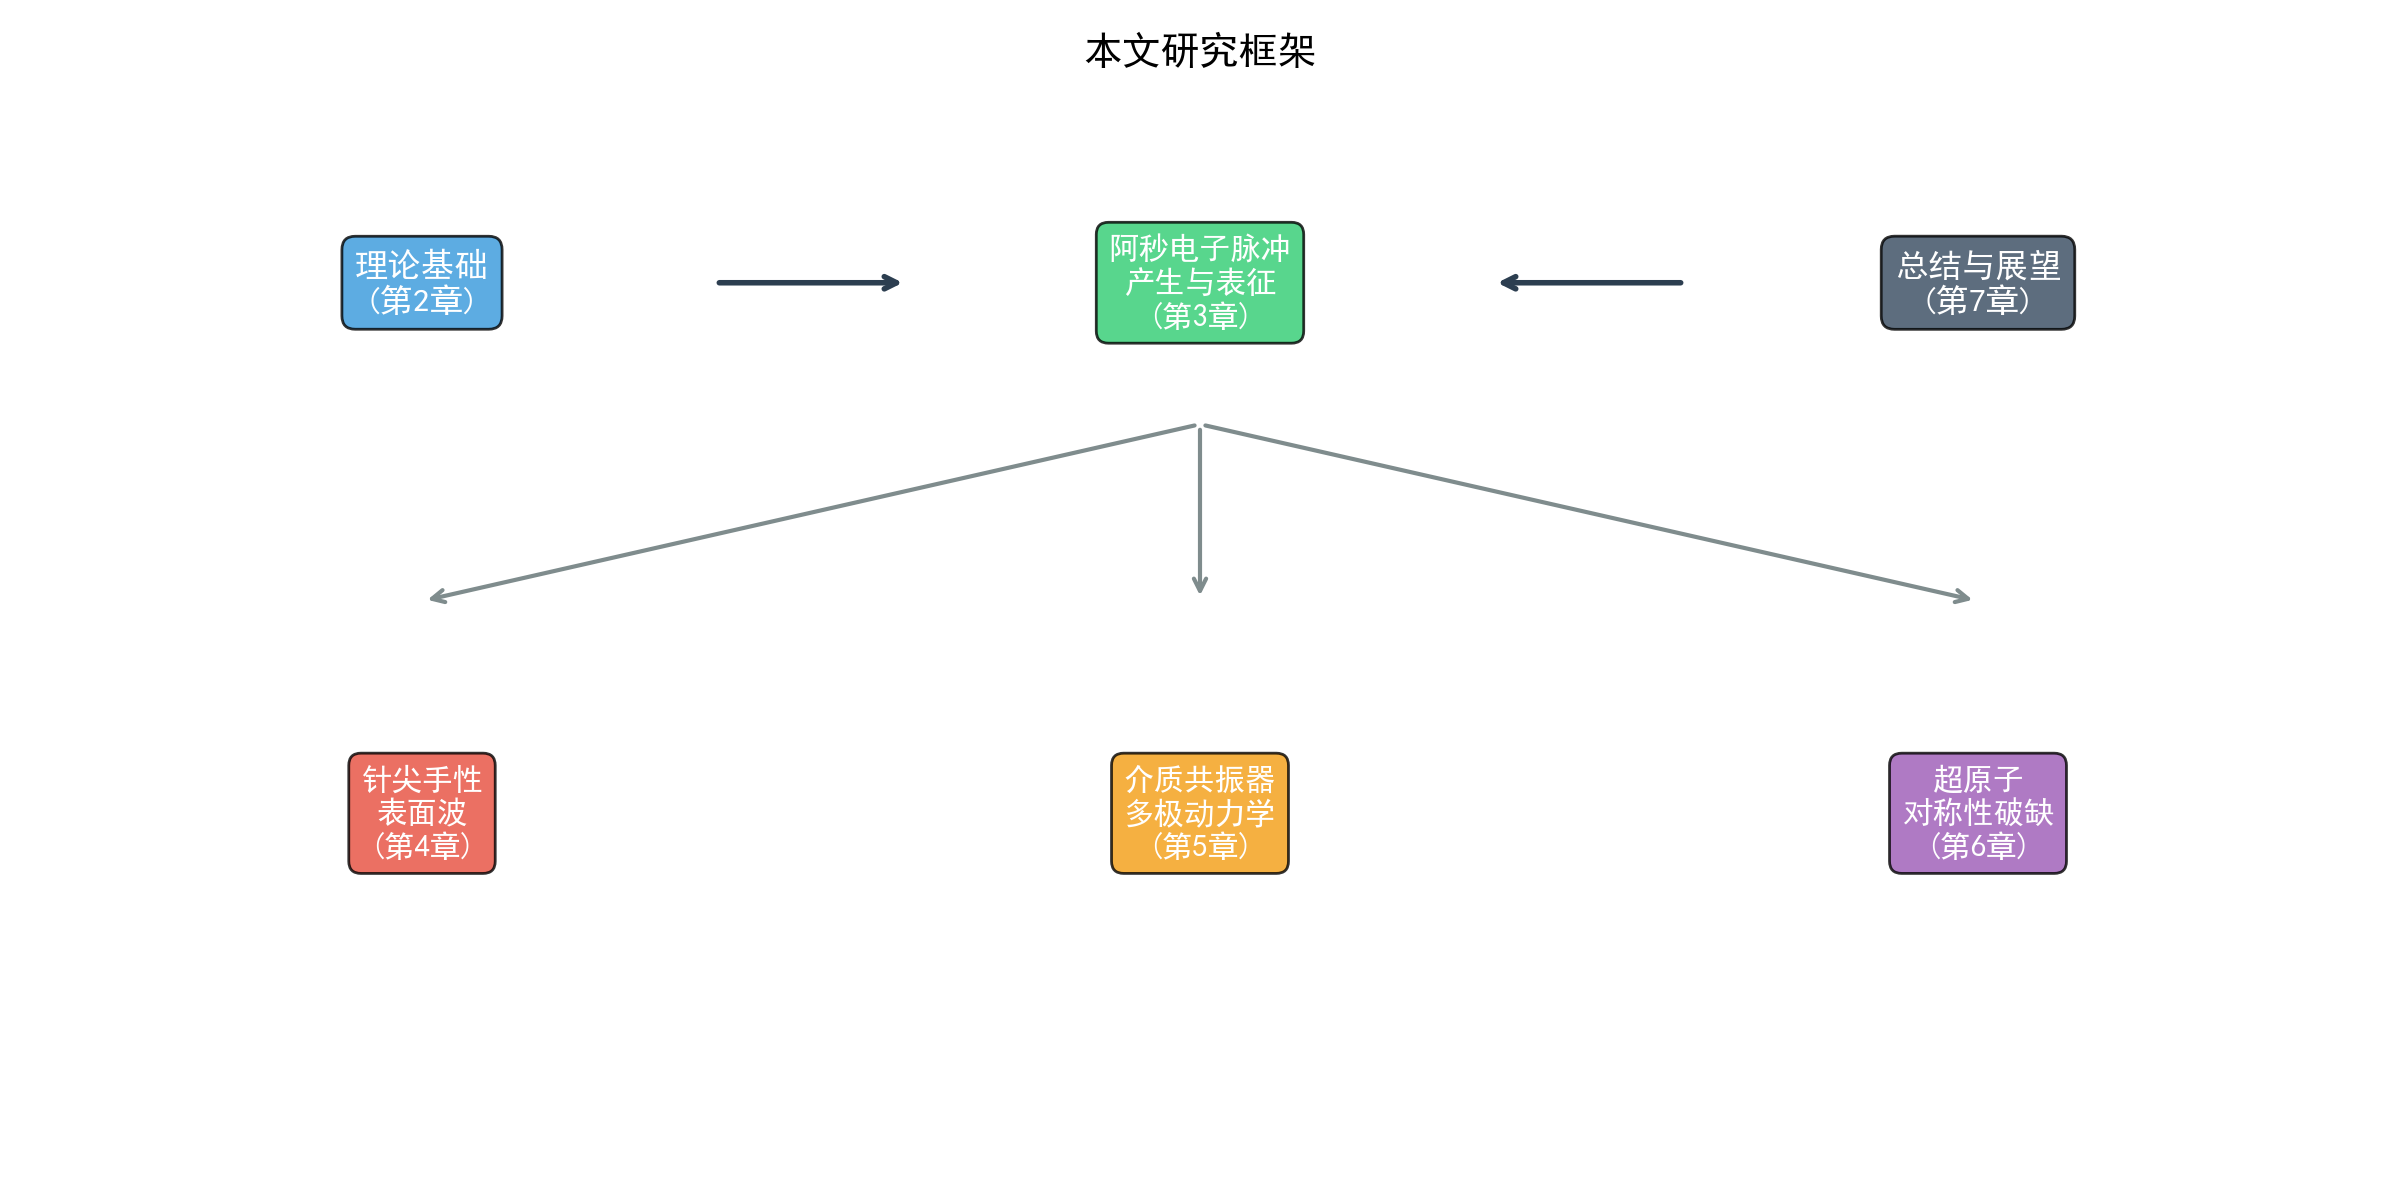
\includegraphics[width=0.9\linewidth]{ch1/fig_framework}
    \caption{\label{fig:ch1-framework} 本文研究框架。从理论基础出发，发展阿秒电子脉冲产生方法，进而应用于三类纳米光子系统（针尖、共振器、超原子）的亚周期动力学研究。}
\end{figure}

\section{本文主要研究内容与章节安排}
\label{sec:outline}

本文共分为七章，各章内容安排如下：

第一章为绪论，介绍研究背景、超快电子显微术和阿秒科学的发展历程，提出本文的科学问题。

第二章为理论基础，系统阐述电子波函数的光场调制机制、时间Talbot效应与阿秒脉冲形成的物理图像、高次谐波产生的三步模型、以及电子能量损失谱在近场成像中的应用原理。

第三章介绍阿秒电子脉冲的产生与表征方法，包括连续波激光驱动的电子脉冲压缩方案、能量滤波器的对比度增强机制、时间扫描与延迟控制的实现方式、以及时间分辨率的标定方法。

第四章至第六章分别展示三类纳米光子系统的实验研究结果：针尖纳米结构的手性表面波动力学、介质纳米共振器的多极模式干涉、以及多天线超原子的对称性破缺响应。

第七章总结全文工作，归纳主要创新点，并对阿秒电子显微术的未来发展方向进行展望。


% ===== 第2章 理论基础 =====
% 第2章 理论基础
\chapter{理论基础}
\label{chap:theory}

本章系统阐述阿秒电子显微术所涉及的核心物理原理，包括电子波函数的光场调制机制、时间Talbot效应与阿秒脉冲形成、高次谐波产生原理、以及电子能量损失谱在近场成像中的应用。

\section{电子波函数的光场调制}
\label{sec:electron-modulation}

\subsection{自由电子在光场中的有质动力相互作用}
\label{subsec:ponderomotive}

当电子束穿越电磁场时，电子波函数会受到场的空间和时间周期性调制。在有质动力（ponderomotive）近似下，电子感受到的等效势能与光场强度的空间梯度成正比：

\begin{equation}
    \label{eq:ponderomotive}
    U_p(\mathbf{r}, t) = \frac{e^2}{4 m_e \omega^2} |\mathbf{E}(\mathbf{r}, t)|^2
\end{equation}

其中$e$为电子电荷，$m_e$为电子质量，$\omega$为光场角频率，$\mathbf{E}$为电场强度。

当电子以速度$v_z$穿越驻波场时，在电子的共动坐标系中，空间周期性转化为时间周期性，电子波函数获得与光子能量$\hbar\omega$对应的能量侧带。量子力学上，这一过程可以用电子与光子间的能量交换描述：

\begin{equation}
    \label{eq:sideband}
    |\psi\rangle = \sum_{n=-\infty}^{\infty} J_n(2|g|) \, |E_0 + n\hbar\omega\rangle
\end{equation}

其中$J_n$为$n$阶贝塞尔函数，$g$为耦合强度参数，$E_0$为电子初始动能，$n\hbar\omega$为第$n$阶侧带的能量偏移。耦合强度$|g|$与光场强度和相互作用长度成正比。

\subsection{能量调制的演化}
\label{subsec:energy-modulation}

初始的正弦能量调制在自由空间传播过程中经历色散演化。在近轴近似下，电子波包的纵向相移与传播距离$z$的关系为：

\begin{equation}
    \label{eq:phase-evolution}
    \phi_n(z) = \frac{n^2 (\hbar\omega)^2}{2 E_0} \cdot \frac{z}{\hbar v_z}
\end{equation}

这一相位演化导致不同阶侧带之间的干涉，使得电子的时间分布（即概率密度沿时间轴的投影）随传播距离发生周期性变化。这正是时间Talbot效应的物理起源。

\section{时间Talbot效应与阿秒脉冲形成}
\label{sec:talbot}

\subsection{经典Talbot效应的回顾}
\label{subsec:classical-talbot}

经典Talbot效应是指：当相干光照射周期性光栅时，在光栅后方特定距离处会出现光栅像的自再现。这一现象最早由Talbot于1836年发现。自再现距离（Talbot距离）为：

\begin{equation}
    \label{eq:talbot-classical}
    z_T = \frac{2 d^2}{\lambda}
\end{equation}

其中$d$为光栅周期，$\lambda$为光波长。

\subsection{时间域Talbot效应}
\label{subsec:temporal-talbot}

Tsarev等人\cite{Tsarev2021}将经典Talbot效应推广到时间域。当电子波函数被激光进行周期性能量调制后，在自由空间传播过程中，不同能量侧带之间的相位演化会导致电子时间分布的自再现。时间Talbot距离为：

\begin{equation}
    \label{eq:talbot-temporal}
    z_T^{\text{time}} = \frac{2 E_0^2}{(\hbar\omega)^2} \cdot \frac{\lambda_e}{2\pi}
\end{equation}

其中$\lambda_e = h / \sqrt{2 m_e E_0}$为电子的德布罗意波长。在$z = z_T^{\text{time}} / 2$处（半Talbot距离），电子的时间分布压缩为原始周期$T = 2\pi/\omega$内的一系列窄脉冲，即阿秒电子脉冲串。图\ref{fig:ch2-talbot}示意了这一过程。

\begin{figure}[htbp]
    \centering
    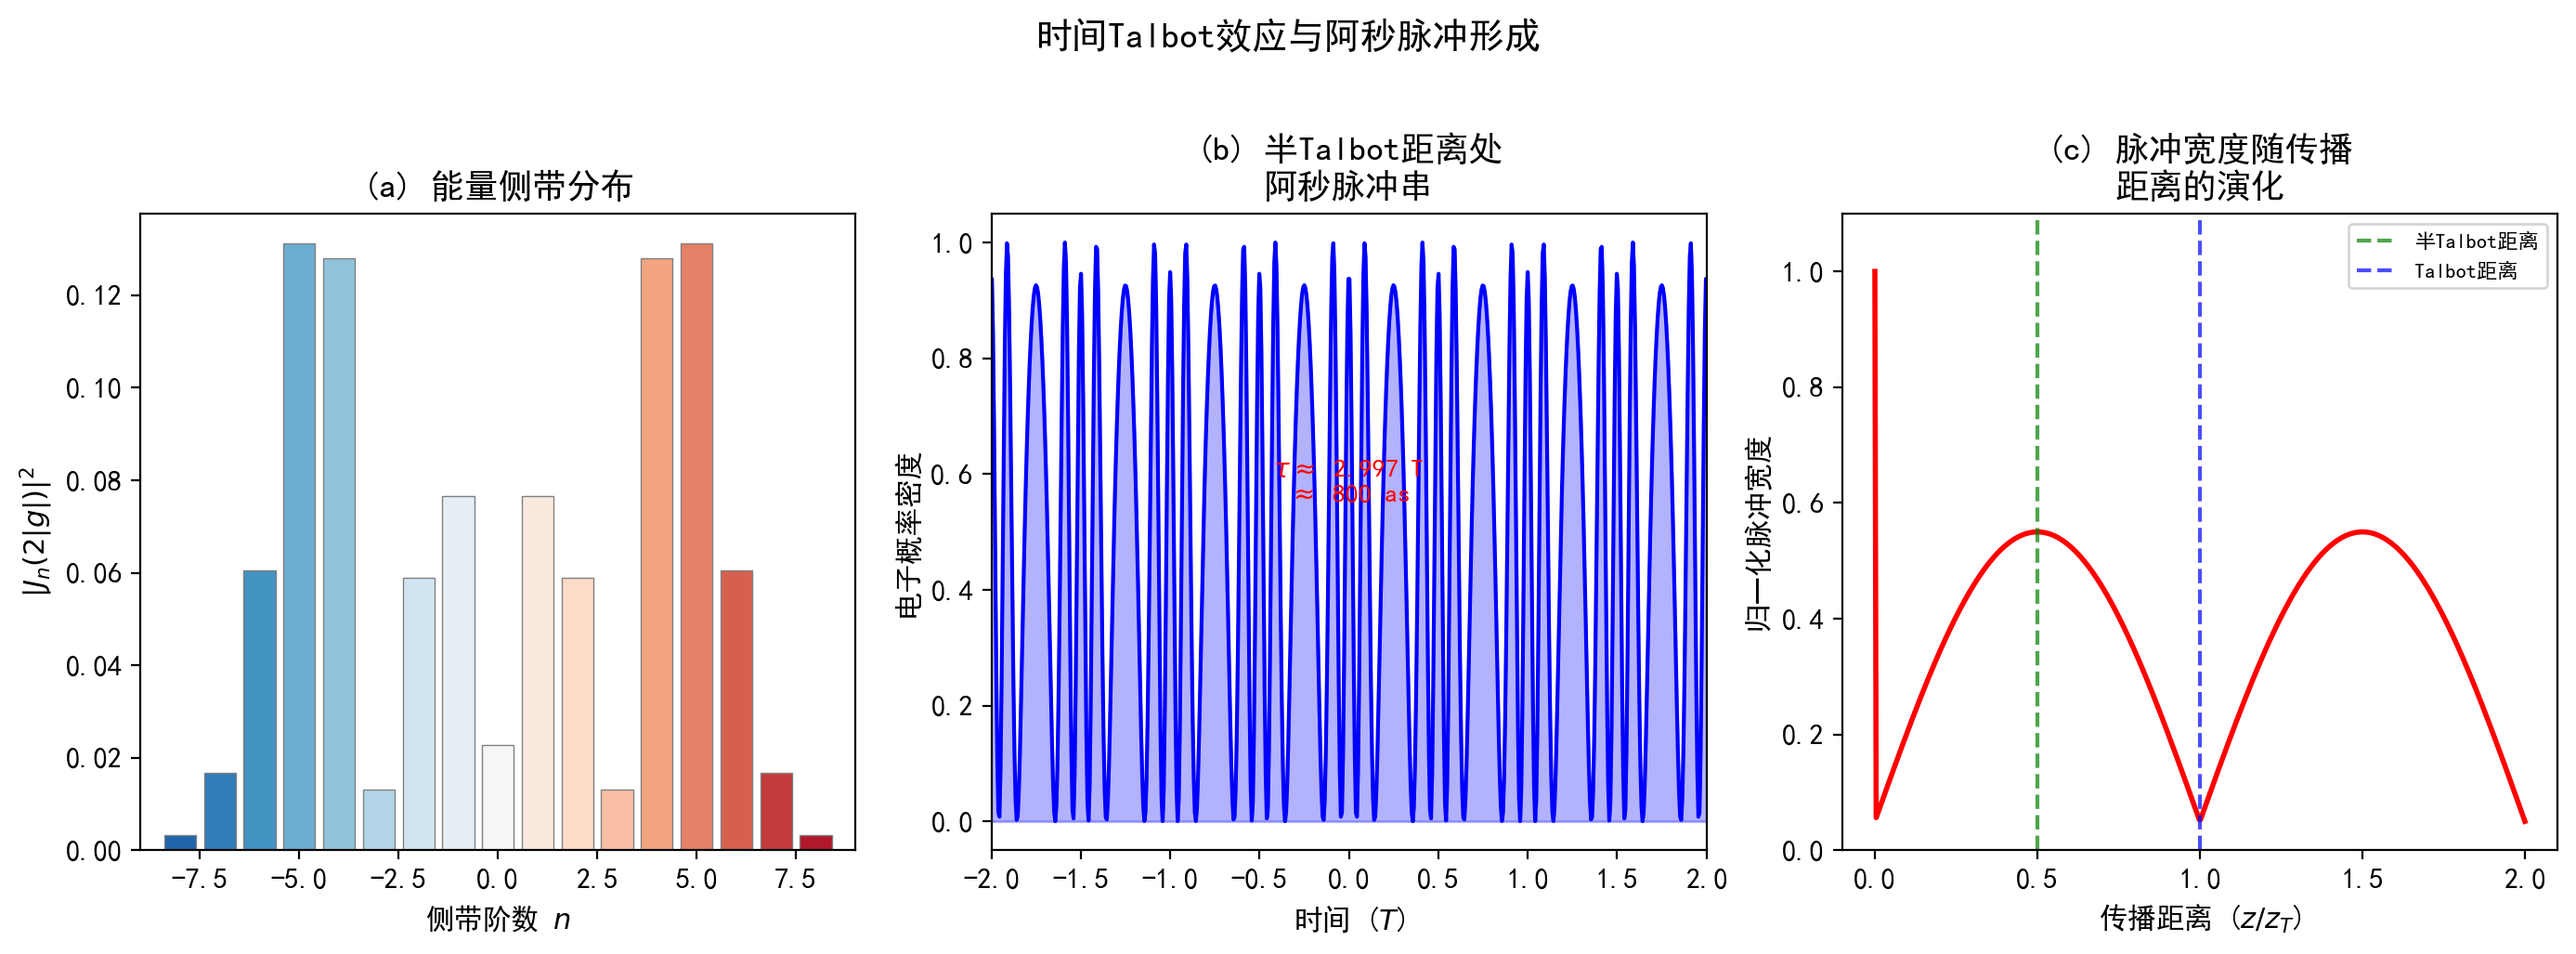
\includegraphics[width=0.9\linewidth]{ch2/fig_talbot}
    \caption{\label{fig:ch2-talbot} 时间Talbot效应产生阿秒电子脉冲串的原理。(a) 初始能量调制使电子波函数获得周期性侧带；(b) 在半Talbot距离处，各侧带的相长干涉形成阿秒脉冲；(c) 单个脉冲的时间宽度由调制深度和侧带阶数共同决定。}
\end{figure}

\subsection{脉冲宽度的定量估计}
\label{subsec:pulse-duration}

在调制深度$|g|$足够大时（$|g| \gg 1$），阿秒脉冲的时间宽度（FWHM）可近似为：

\begin{equation}
    \label{eq:pulse-width}
    \tau_{\text{as}} \approx \frac{T}{2\pi |g|} = \frac{1}{|g| \cdot \omega}
\end{equation}

对于800\,nm波长的连续波激光（$\omega \approx 2.4 \times 10^{15}\;\text{rad/s}$）和典型调制深度$|g| \approx 3$，脉冲宽度约为$\SI{800}{as}$。增大激光功率可提高$|g|$，从而进一步缩短脉冲宽度。

\section{高次谐波产生的三步模型}
\label{sec:hhg}

\subsection{三步模型的基本图像}
\label{subsec:three-step}

Corkum\cite{Corkum1993}提出的三步模型将高次谐波产生过程分解为以下三个阶段（如图\ref{fig:ch2-hhg}所示）：

\textbf{第一步：隧道电离}。强激光场使原子势垒发生倾斜，价电子通过量子隧穿效应逃离原子实的束缚。电离概率由Landau-Zener公式或ADK（Ammosov-Delone-Krainov）理论描述。

\textbf{第二步：自由电子的加速运动}。电离后的电子在激光场中被加速，获得额外的动能。电子的运动轨迹由激光场的相位决定。根据经典力学，在激光场相位$\phi_0$处电离的电子，其返回时间$t_r$和返回动能$E_{\text{kin}}$满足：

\begin{equation}
    \label{eq:return-energy}
    E_{\text{kin}}(\phi_0) = 2 U_p \left[\sin(\omega t_r - \phi_0) - \sin(-\phi_0)\right]^2
\end{equation}

其中$U_p = e^2 E_0^2 / (4 m_e \omega^2)$为有质动力能量。最大返回动能为$3.17\,U_p$，对应截止频率$\hbar\omega_{\text{cutoff}} = I_p + 3.17\,U_p$（$I_p$为电离能）。

\textbf{第三步：复合辐射}。返回的电子与母离子复合，将获得的动能和电离能以高能光子的形式辐射。辐射光子的能量为$\hbar\omega_n = n\hbar\omega_0$，其中$n$为谐波阶数。

\begin{figure}[htbp]
    \centering
    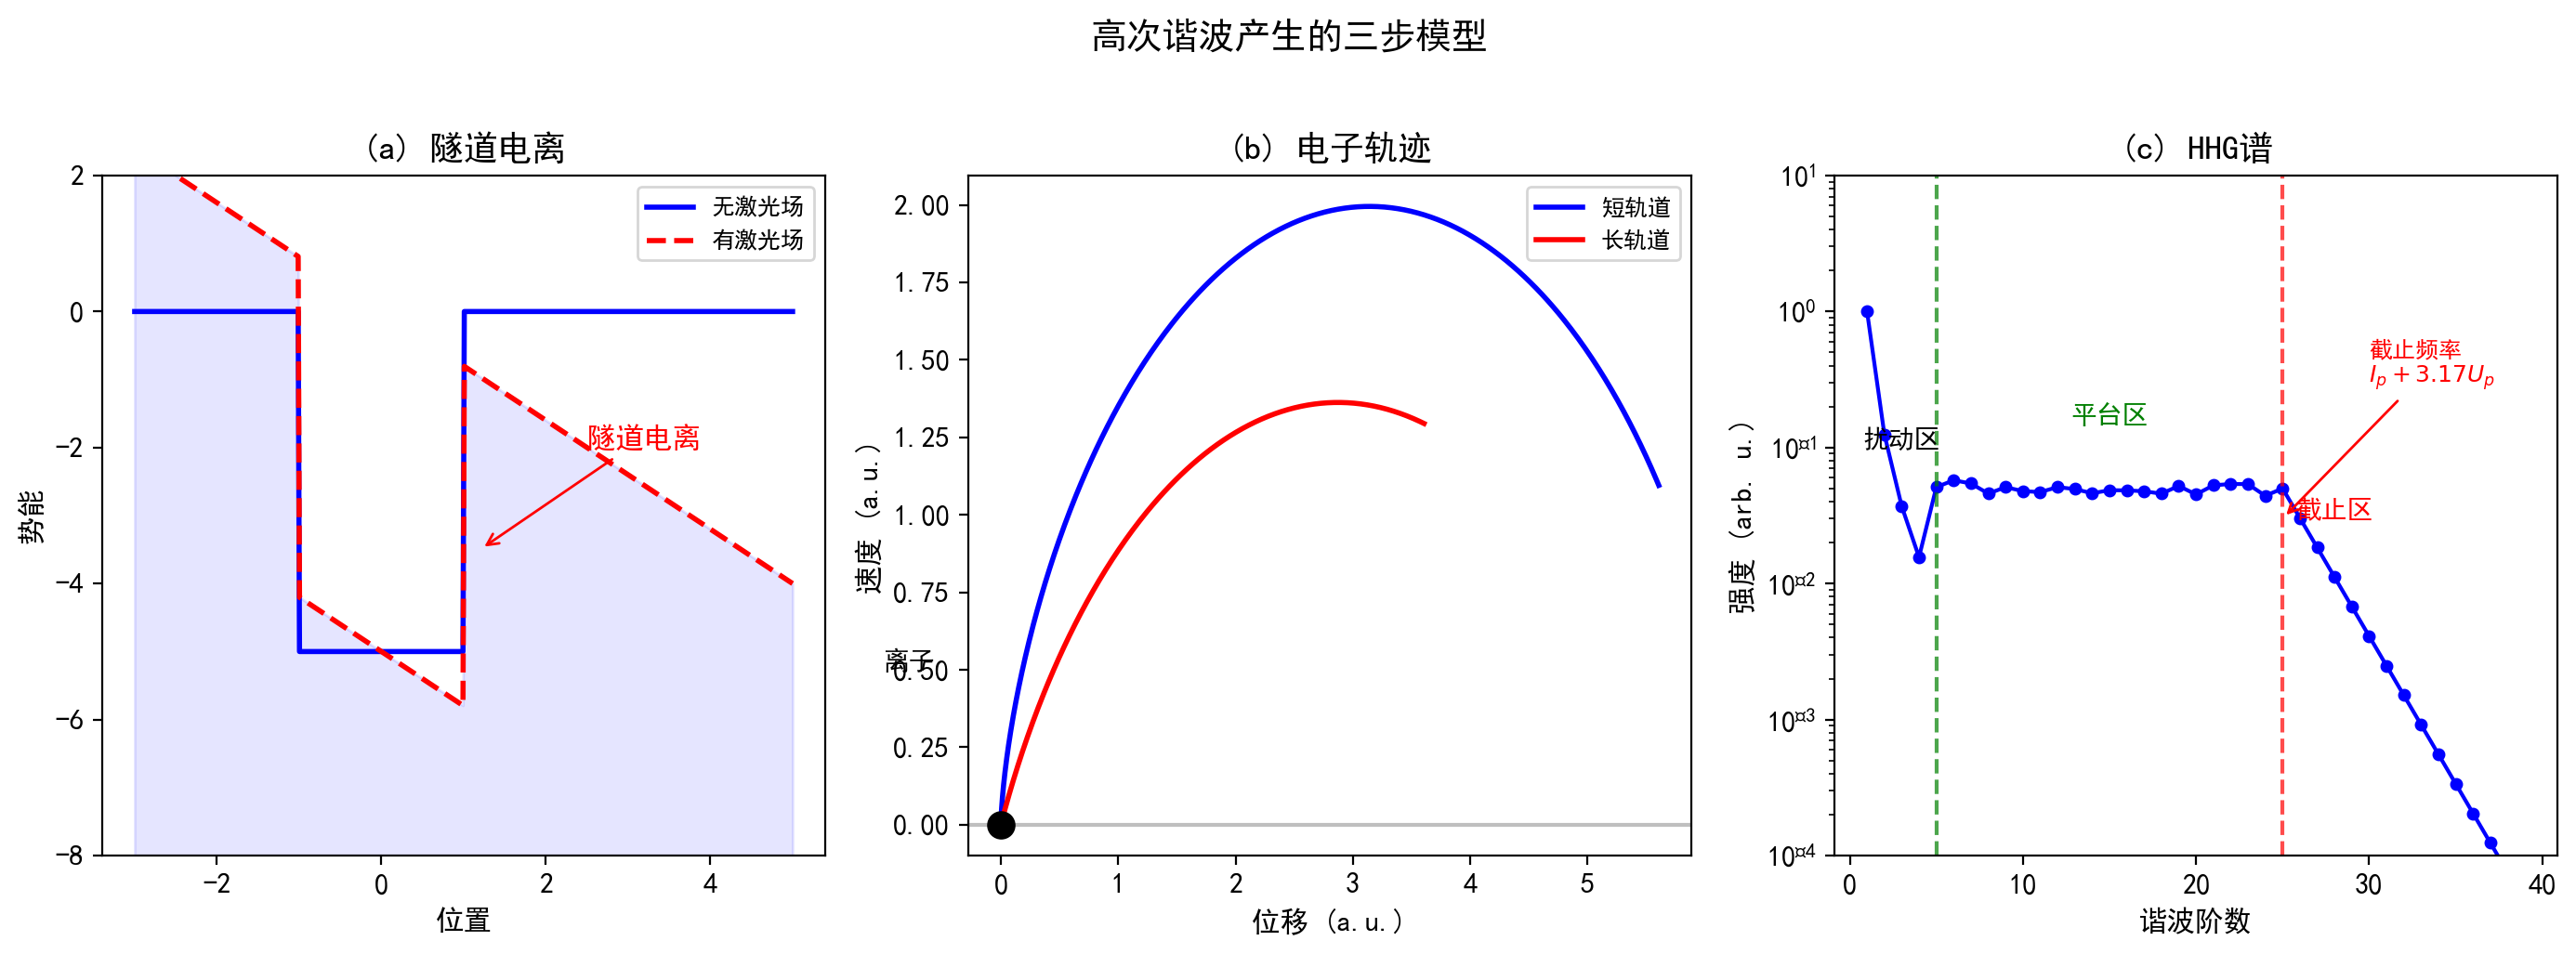
\includegraphics[width=0.85\linewidth]{ch2/fig_hhg_model}
    \caption{\label{fig:ch2-hhg} 高次谐波产生的三步模型。(a) 原子势在强激光场作用下发生倾斜；(b) 电子隧道电离后被激光场加速；(c) 电子返回母离子并复合辐射出高能光子。}
\end{figure}

\subsection{HHG平台区与阿秒脉冲产生}
\label{subsec:hhg-plateau}

HHG谱具有典型的平台区特征：在低阶谐波区，强度随阶数快速下降；进入平台区后，谐波强度在很宽的能量范围内近似保持恒定；在截止频率处急剧下降。Antoine等人\cite{Antoine1996}指出，平台区内大量等间距谐波的相干叠加可以产生阿秒脉冲串。对于理想的平台区（谐波从$q_{\min}$到$q_{\max}$，等间距，等振幅），合成脉冲的时间宽度为：

\begin{equation}
    \label{eq:atto-train}
    \tau = \frac{2\pi}{(q_{\max} - q_{\min})\omega}
\end{equation}

覆盖的谐波阶数越多，脉冲越短。这一原理是本文理解阿秒时间尺度的基础。

\section{电子能量损失谱与近场成像}
\label{sec:eels}

\subsection{电子能量损失谱的基本原理}
\label{subsec:eels-principle}

高速电子穿过薄样品时，会通过库仑相互作用与样品中的电磁场发生能量交换。电子能量损失谱（electron energy-loss spectroscopy, EELS）记录入射电子在透射过程中损失的能量分布。损失的能量$\Delta E$反映了电子与样品中特定激发模式（等离激元、声子、带间跃迁等）的耦合强度。

\subsection{近场成像的对比度机制}
\label{subsec:nearfield-contrast}

在阿秒电子显微术中，能量滤波器选择获得了特定能量增益$\Delta E > E_{\text{cut}}$的电子。这些电子在与近场相互作用过程中获得了净能量转移。能量增益的空间分布直接反映了纳米结构近场的振幅和相位信息。

与传统的EELS不同，阿秒场周期对比度成像的信号来源是电子与近场中光子态的受激能量交换（photon-induced near-field electron microscopy, PINEM），其能量变化为离散的光子能量$\hbar\omega$的整数倍。通过扫描激光-电子之间的时间延迟$\Delta t$，可以获得近场随时间演化的"电影"。

\begin{figure}[htbp]
    \centering
    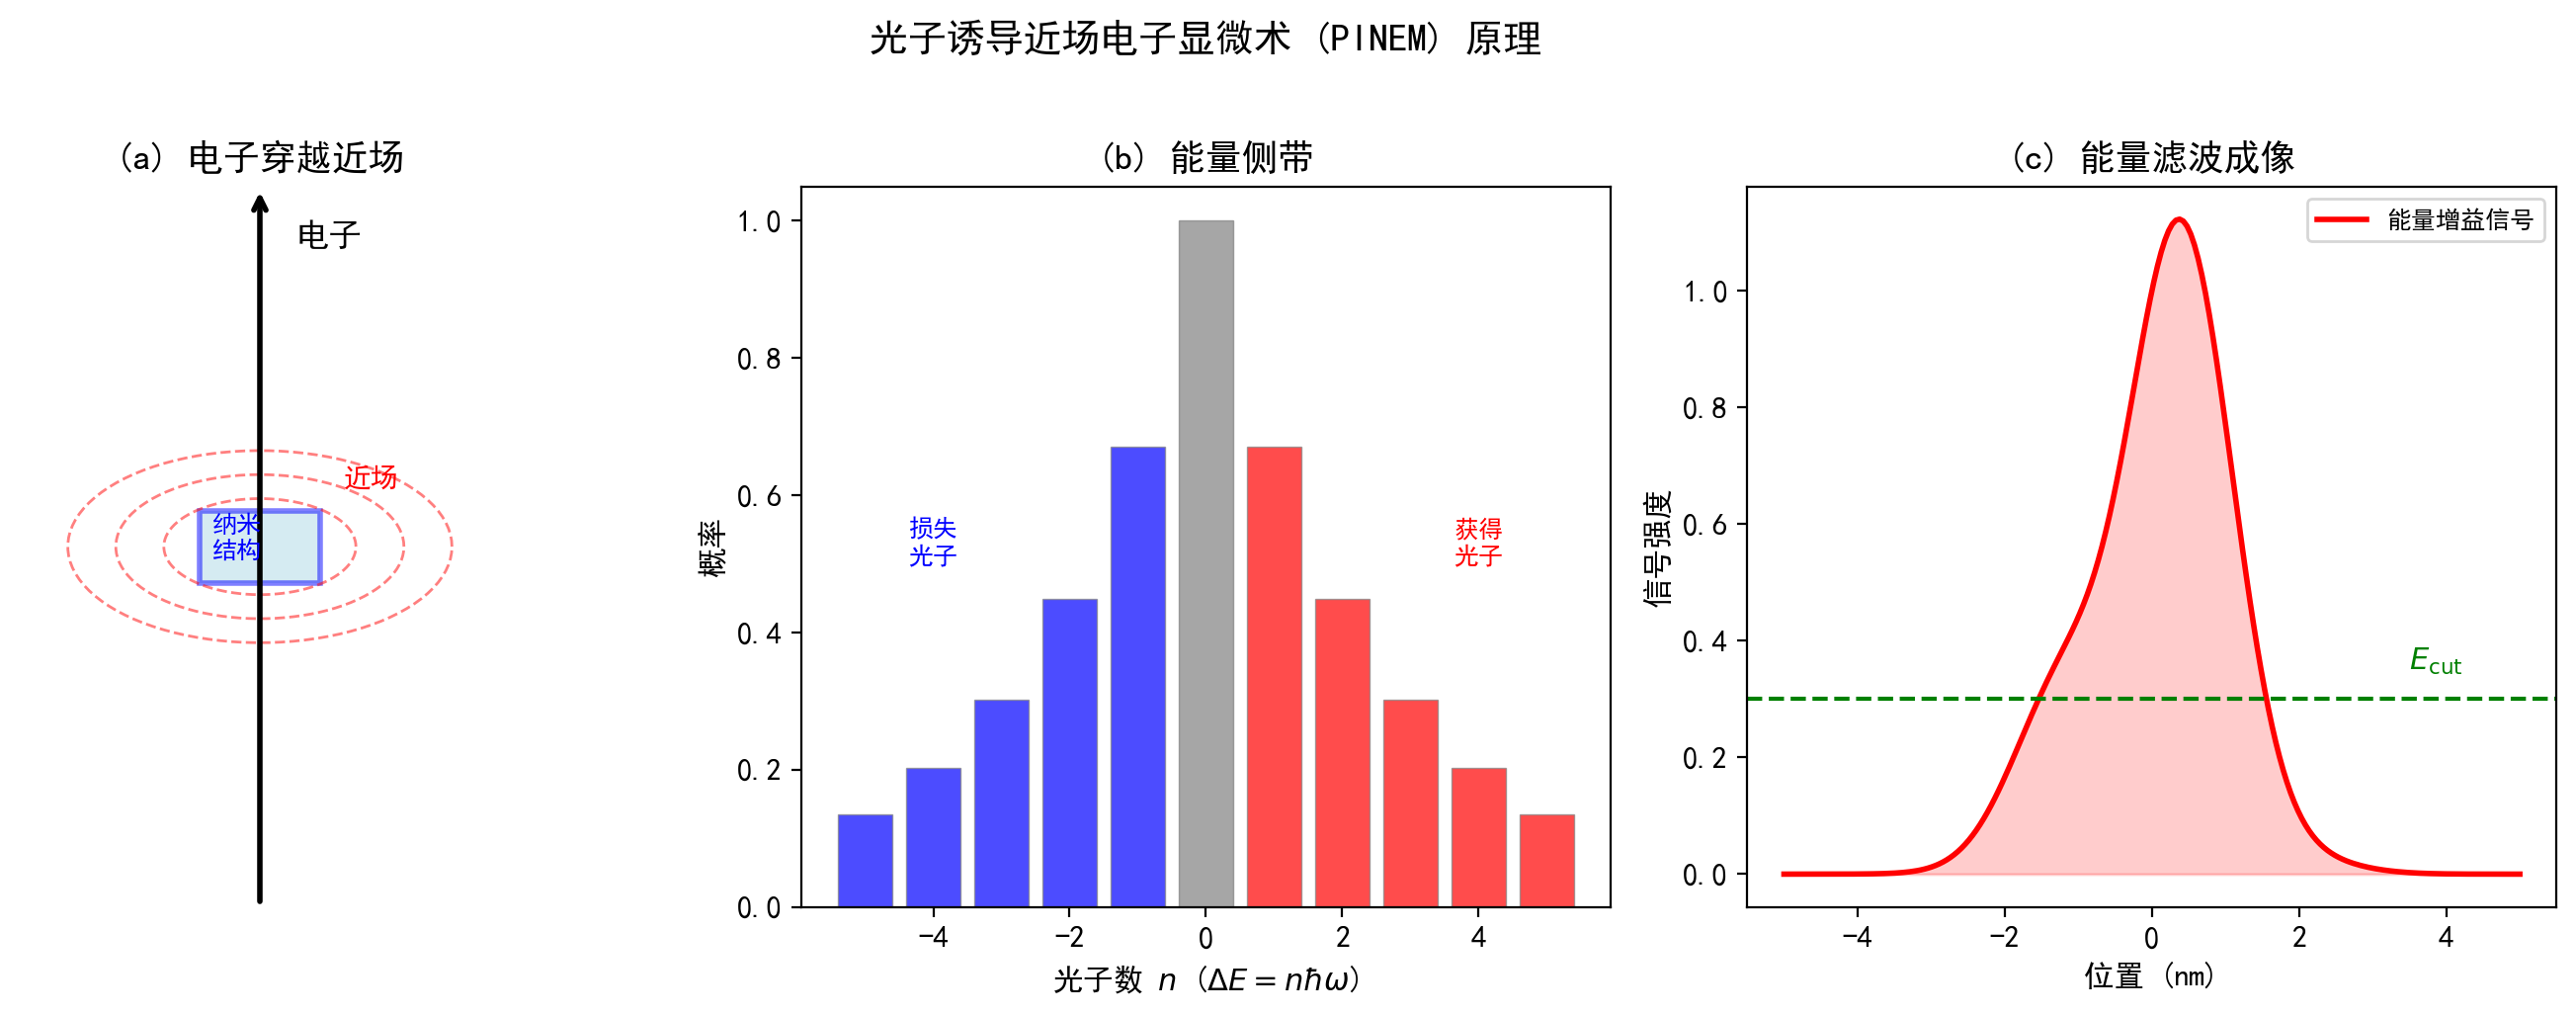
\includegraphics[width=0.85\linewidth]{ch2/fig_pinem}
    \caption{\label{fig:ch2-pinem} 光子诱导近场电子显微术（PINEM）的原理。(a) 电子穿过纳米结构的近场区域；(b) 电子与光场交换整数个光子能量，形成能量侧带；(c) 能量滤波后获得近场分布的空间映射。}
\end{figure}

\section{本章小结}
\label{sec:theory-summary}

本章介绍了阿秒电子显微术的理论基础。电子波函数在光场中的有质动力调制产生周期性能量侧带，通过时间Talbot效应在自由空间传播中演化形成阿秒电子脉冲串。高次谐波产生的三步模型为理解阿秒时间尺度提供了物理图像。电子能量损失谱与PINEM机制为近场成像提供了对比度来源。上述理论构成本文实验研究的基础框架。


% ===== 第3章 阿秒电子脉冲的产生与表征方法 =====
% 第3章 阿秒电子脉冲的产生与表征方法
\chapter{阿秒电子脉冲的产生与表征方法}
\label{chap:method}

本章介绍实验系统的搭建与关键参数的表征，包括透射电子显微镜的光学集成方案、连续波激光驱动的阿秒电子脉冲产生、能量滤波器的优化配置、以及时间分辨率的标定方法。

\section{实验系统概述}
\label{sec:exp-overview}

% 实验系统整体介绍：TEM + CW激光 + 能量滤波器

\begin{figure}[htbp]
    \centering
    % TODO: 从素材库提取实验系统示意图
    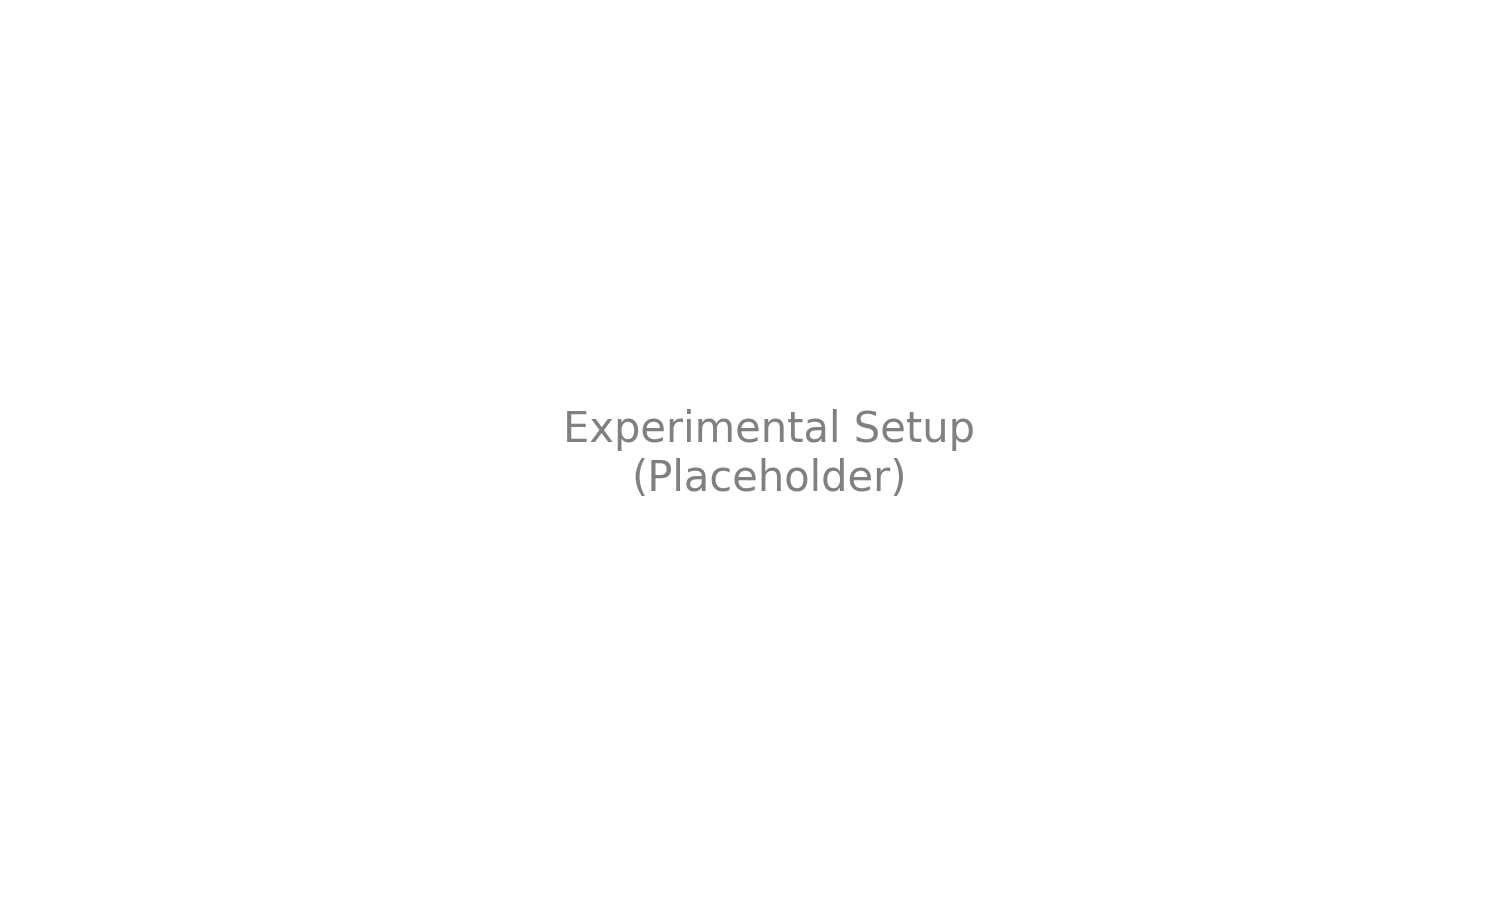
\includegraphics[width=0.9\linewidth]{ch3/fig_exp_setup}
    \caption{\label{fig:ch3-setup} 阿秒电子显微术实验系统示意图。连续波激光（红色光路）同时照射压缩膜和样品。电子束（蓝色箭头）穿越压缩膜获得能量调制，在样品平面处形成阿秒脉冲串。能量滤波器选择特定能量侧带的电子成像。}
\end{figure}

\section{连续波激光驱动的电子脉冲压缩}
\label{sec:cw-compression}

% 3.2 CW激光参数选择
% 3.2.1 压缩膜（Si3N4）的制备与集成
% 3.2.2 激光-电子对准方案
% 3.2.3 调制深度|g|的测量与优化

\section{能量滤波器的对比度增强}
\label{sec:energy-filter}

% 3.3 能量滤波器配置
% 3.3.1 GIF（Gatan Imaging Filter）的参数设置
% 3.3.2 能量窗口宽度的选择
% 3.3.3 背景扣除与信噪比优化

\section{时间扫描与延迟控制}
\label{sec:delay-control}

% 3.4 时间延迟的精密控制
% 3.4.1 压电平移台的校准
% 3.4.2 时间零点的确定
% 3.4.3 相位锁定与稳定性

\section{时间分辨率的标定}
\label{sec:resolution-calibration}

% 3.5 时间分辨率的实验标定
% 3.5.1 从能量谱推算脉冲宽度
% 3.5.2 空间分辨率的测量（PSF法）
% 3.5.3 系统误差分析

\begin{table}[htbp]
    \caption{\label{tab:ch3-params} 实验系统关键参数}
    \begin{tabularx}{\linewidth}{c|X<{\centering}}
        \hline
        参数 & 数值 \\ \hline
        电子能量 $E_0$ & \SI{183}{keV} \\ \hline
        激光波长 $\lambda$ & \SI{785(5)}{nm} \\ \hline
        激光功率 $P$ & \SI{300(10)}{mW} \\ \hline
        脉冲宽度（FWHM）& \SI{800(50)}{as} \\ \hline
        空间分辨率 & \SI{50(10)}{nm} \\ \hline
        时间扫描步长 & $\sim$\SI{3}{as} \\ \hline
        能量滤波窗口 & $\Delta E > $\SI{1}{eV} \\ \hline
    \end{tabularx}
\end{table}

\section{本章小结}
\label{sec:method-summary}

本章介绍了阿秒电子显微术实验系统的搭建与关键参数表征。系统以连续波激光驱动，在常规TEM中实现了$\sim$\SI{800}{as}的时间分辨率和$\sim$\SI{50}{nm}的空间分辨率，为后续的纳米光子系统亚周期动力学研究提供了可靠的实验基础。


% ===== 第4章 针尖纳米结构的手性表面波动力学 =====
% 第4章 针尖纳米结构的手性表面波动力学
\chapter{针尖纳米结构的手性表面波动力学}
\label{chap:result1}

\section{引言}
\label{sec:r1-intro}

% 纳米针尖作为表面等离激元研究的经典模型体系
% 手性光-物质相互作用的基本概念
% 本章研究目标：利用阿秒电子显微术观测针尖上手性表面波的亚周期动力学

\section{纳米针尖的制备与表征}
\label{sec:r1-fabrication}

% 钨针尖的FIB加工
% 狭缝结构的引入
% SEM表征

\begin{figure}[htbp]
    \centering
    % 占位符：用户实验数据图
    \fbox{\parbox{0.8\linewidth}{\centering\vspace{3cm} 图4-1：钨纳米针尖SEM图像\\（实验数据待插入）\vspace{3cm}}}
    \caption{\label{fig:ch4-tip} 狭缝修饰的钨纳米针尖。(a) 全景SEM图像；(b) 针尖顶端狭缝结构的高倍率图像。}
\end{figure}

\section{圆偏振光激发的手性响应}
\label{sec:r1-chiral}

% 左旋和右旋圆偏振光分别激发
% 方向性表面波的产生
% 手性选择性机制：自旋-轨道耦合

\section{亚周期时间分辨测量}
\label{sec:r1-temporal}

% 时间延迟扫描数据
% 表面波传播方向的手性控制
% 相位速度测量

\begin{figure}[htbp]
    \centering
    % 占位符：用户实验数据图
    \fbox{\parbox{0.8\linewidth}{\centering\vspace{3cm} 图4-2：手性表面波时间分辨测量\\（实验数据待插入）\vspace{3cm}}}
    \caption{\label{fig:ch4-chiral} 圆偏振光激发下手性表面波的时间分辨测量。(a-b) 左旋（LCP）和右旋（RCP）圆偏振光激发下的能量滤波图像；(c-e) 选定延迟时刻的场演化。}
\end{figure}

\section{表面波传播特性的定量分析}
\label{sec:r1-analysis}

% 相位速度的超光速特征
% 近场衰减距离
% 左旋-右旋之间$\sim$1.8\,fs的延迟

\section{本章小结}
\label{sec:r1-summary}

本章利用阿秒电子显微术研究了狭缝修饰钨针尖上的手性表面波动力学。实验结果表明，圆偏振光的偏振手性可以通过自旋-轨道耦合机制控制表面波的传播方向，在亚周期时间尺度上实现了对纳米光子激发的方向性操控。左旋和右旋激发图案之间存在$\sim$\SI{1.8}{fs}的时间延迟，反映了手性表面波的矢量特征。


% ===== 第5章 介质纳米共振器中的多极模式动力学 =====
% 第5章 介质纳米共振器中的多极模式动力学
\chapter{介质纳米共振器中的多极模式动力学}
\label{chap:result2}

\section{引言}
\label{sec:r2-intro}

% 介质纳米共振器作为纳米光子学的核心构件
% Mie共振理论简介
% 偶极与四极模式的同时激发与干涉

\section{介质纳米共振器的设计与制备}
\label{sec:r2-design}

% 硅膜上的狭缝共振器设计
% FIB加工参数
% 结构表征

\begin{figure}[htbp]
    \centering
    % 占位符：用户实验数据图
    \fbox{\parbox{0.8\linewidth}{\centering\vspace{3cm} 图5-1：介质纳米共振器\\（实验数据待插入）\vspace{3cm}}}
    \caption{\label{fig:ch5-resonator} 200\,nm厚硅膜上的狭缝共振器。(a) SEM图像；(b) 几何尺寸标注。}
\end{figure}

\section{偶极与四极模式的时域分辨}
\label{sec:r2-multipolar}

% 实验测量的空间-时间数据
% SVD分析确认两个主导模式
% 偶极和四极模式之间的相位延迟

\section{内部波前的传播速度测量}
\label{sec:r2-wavefront}

% 狭缝内传播波前的直接观测
% 相速度与有效折射率的关系
% 亚光速传播的物理机制

\section{数值模拟验证}
\label{sec:r2-simulation}

% FDTD模拟设置
% 模拟与实验的对比
% 模式分析

\begin{figure}[htbp]
    \centering
    % 占位符：用户实验数据图
    \fbox{\parbox{0.8\linewidth}{\centering\vspace{3cm} 图5-2：多极模式时域分辨\\（实验数据待插入）\vspace{3cm}}}
    \caption{\label{fig:ch5-multipolar} 介质纳米共振器的时域分辨测量。(a) 测量的空间-时间能量变化图；(b-c) 选定时刻的场分布；(d) SVD分析的主导模式。}
\end{figure}

\section{本章小结}
\label{sec:r2-summary}

本章研究了硅介质纳米共振器中偶极和四极Mie共振模式的时间干涉动力学。阿秒电子显微术首次在时域直接分辨了两种模式之间的相位延迟，观测到狭缝内亚光速传播的电磁波前。这些结果为Huygens超表面的设计提供了时域层面的物理认知。


% ===== 第6章 对称性破缺的多天线纳米光子响应 =====
% 第6章 对称性破缺的多天线纳米光子响应
\chapter{对称性破缺的多天线纳米光子响应}
\label{chap:result3}

\section{引言}
\label{sec:r3-intro}

% 超原子/超表面的设计原理
% 对称性在纳米光子学中的重要性
% 制造容差对超表面性能的影响

\section{超原子结构与制备}
\label{sec:r3-structure}

% 四个狭缝的zig-zag排列
% 名义上的镜像对称性
% 制备工艺

\begin{figure}[htbp]
    \centering
    % 占位符：用户实验数据图
    \fbox{\parbox{0.8\linewidth}{\centering\vspace{3cm} 图6-1：超原子结构\\（实验数据待插入）\vspace{3cm}}}
    \caption{\label{fig:ch6-meta} zig-zag排列的四狭缝超原子。(a) SEM图像；(b) 几何设计示意图，标注名义对称轴。}
\end{figure}

\section{实验测量结果}
\label{sec:r3-results}

% 振幅图和相位图
% 对称性破缺的直观观察
% 与数值模拟的偏差

\section{对称性破缺的机制分析}
\label{sec:r3-symmetry}

% $\sim$\SI{10}{nm}级别的加工不完美
% 相位差达$\pi/3$的定量分析
% 对电磁能量流的重新导向

\begin{figure}[htbp]
    \centering
    % 占位符：用户实验数据图
    \fbox{\parbox{0.8\linewidth}{\centering\vspace{3cm} 图6-2：对称性破缺测量\\（实验数据待插入）\vspace{3cm}}}
    \caption{\label{fig:ch6-symmetry} 超原子的对称性破缺响应。(a) 振幅图，干涉极大位置相对于对称预测的偏移；(b) 四个位置的时域信号，展示相干但不对称的场振荡。}
\end{figure}

\section{对超表面设计的启示}
\label{sec:r3-implication}

% 加工容差的分析
% 鲁棒性设计策略
% 主动补偿的可能性

\section{本章小结}
\label{sec:r3-summary}

本章研究了四狭缝超原子中结构对称性对电磁响应的影响。实验发现，即使名义上具有镜像对称的结构，$\sim$\SI{10}{nm}级别的加工偏差也足以导致电磁能量流的定向偏转，相位差可达$\pi/3$。这一结果揭示了超表面设计中加工精度与功能确定性之间的定量关系。


% ===== 第7章 总结与展望 =====
% 第7章 总结与展望
\chapter{总结与展望}
\label{chap:conclusion}

\section{本文工作总结}
\label{sec:summary}

本文围绕阿秒电子显微术的核心问题——如何在常规透射电子显微镜中实现亚周期时间分辨的电磁近场成像——开展了系统的研究。主要工作包括：

（1）建立了基于连续波激光驱动的阿秒电子脉冲产生方案。利用有质动力相互作用和时间Talbot效应，在电子波函数中刻印阿秒级时间结构，产生了$\sim$\SI{800}{as}的电子脉冲串。

（2）开发了阿秒场周期对比度成像方法。通过能量滤波器选择光子诱导能量增益的电子，实现了对纳米结构近场的空间分辨和时间分辨同时测量。

（3）在三类纳米光子系统中开展了亚周期动力学研究：针尖结构的手性表面波、介质共振器的多极模式干涉、多天线超原子的对称性破缺。

\section{主要创新点}
\label{sec:innovation}

本文的主要创新点如下：

\begin{enumerate}
    \item 提出了利用连续波激光在常规TEM中产生阿秒电子脉冲的实验方案，无需飞秒激光系统即可实现$\sim$\SI{800}{as}时间分辨率。
    \item 在亚周期时间尺度上观测到了手性表面波的方向性传播，揭示了自旋-轨道耦合在纳米光子激发中的矢量特性。
    \item 直接测量了介质纳米共振器中偶极和四极Mie模式的相对相位延迟，为Huygens超表面的时域设计提供了实验依据。
    \item 定量表征了$\sim$\SI{10}{nm}加工偏差对多天线系统电磁响应对称性的影响，为超表面的制造精度要求提供了参考。
\end{enumerate}

\section{展望}
\label{sec:outlook}

阿秒电子显微术作为一个新兴的研究方向，具有广阔的发展空间。未来的研究方向包括：

（1）\textbf{非重复动力学的单次成像}。目前的CW激光方案仅适用于周期性动力学过程。通过单周期束控技术\cite{Baum2007}或三波有质动力偏转方案\cite{Morimoto2020}，有望实现对非重复事件（如相变、随机开关）的阿秒时间分辨成像，代价是信噪比降低$\sim$100倍。

（2）\textbf{空间分辨率的提升}。当前$\sim$\SI{50}{nm}的空间分辨率受能量滤波器狭缝宽度限制。通过像差校正光学系统\cite{Morimoto2018}，有望将空间分辨率推进至$<\SI{10}{nm}$。

（3）\textbf{矢量场重构}。目前的技术测量的是电场沿电子轨迹的投影，而非完整的三维矢量场。通过倾转系列断层扫描方法，可以重构矢量场分布，代价是采集时间增加$\sim$10倍。

（4）\textbf{应用领域的拓展}。阿秒电子显微术有望应用于拓扑光子结构的近场表征、二维材料中的超快载流子动力学、以及量子材料中的相干声子激发等前沿问题。


% ===== 后置部分 =====
\poststyle
\cleardoublepage
\begingroup
    \printbibliography[title={参考文献}]
\endgroup

\cleardoublepage
\chaptercenter{作者简历}

简历内容

\cleardoublepage
\chapternonum{攻读博士学位期间取得的科研成果}

\section*{期刊论文}
\begin{enumerate}
    \item 论文列表（待填写）
\end{enumerate}

\section*{会议报告}
\begin{enumerate}
    \item 报告列表（待填写）
\end{enumerate}


\end{document}
